\chapter{序論}
\section{背景}
近年,様々なセンサを用いた移動ロボットの自律移動に関する研究が盛んに行われており,
その中でカメラ画像を用いてロボットへ自律移動を行わせる研究も行われている.
%\index{うえだ@上田}
%例として,\cite{上田2015gihyo,ueda2015,上田2015jsai}がある.
Bojaskiら\cite{Nvidia}は
Fig. \ref{fig::nvidia}で示す方法で,人間のハンドル操作によるステアリングの角度の模倣学習を行い,
画像を用いて走行を行う方法を提案した.

\begin{figure}[h]
    \centering
    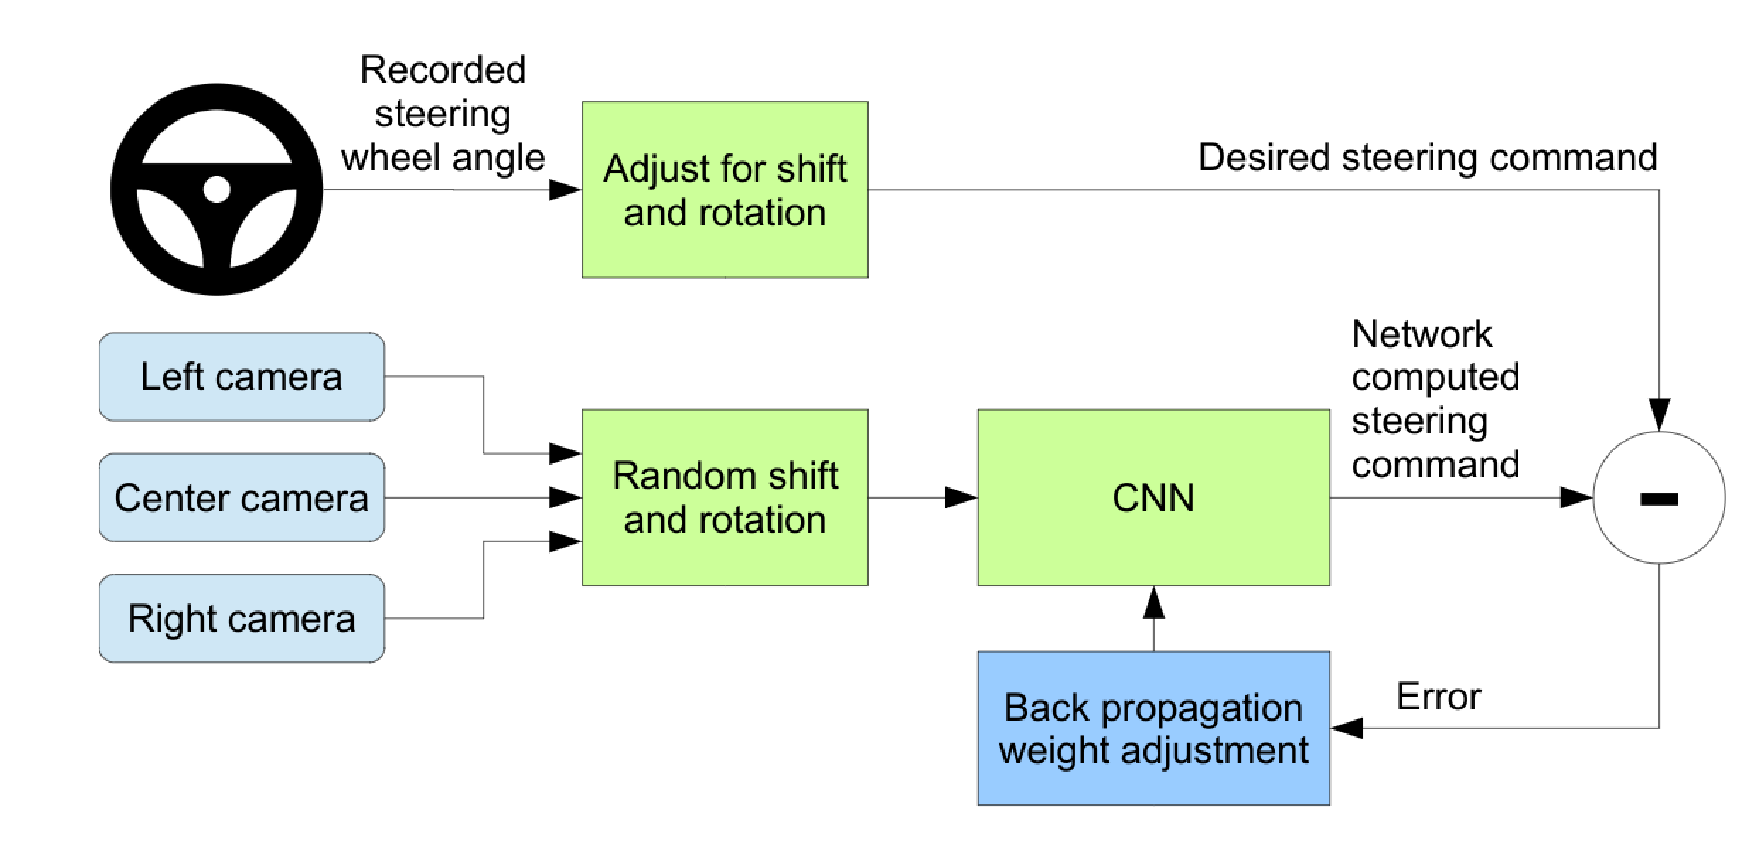
\includegraphics[width = 13cm]{./figs/EndtoEnd_Learning_for_Self-Driving_Cars.pdf}
    \caption{Training the neural network from \cite{Nvidia}}
    \label{fig::nvidia}
\end{figure}

\newpage
本研究室においても岡田ら\cite{okada}によってFig. \ref{fig::okada_sys}に示すように
LiDAR,オドメトリを入力とした地図べースの制御器の出力と
その際に取得したカメラ画像を訓練データとして用いることで,\ref{fig::okada}
経路追従行動を模倣が可能であること
を確認した.
\begin{figure}[h]
    \centering
    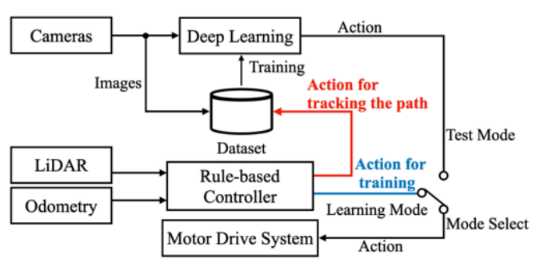
\includegraphics[width = 10cm]{./figs/okada_sys.png}
    \caption{Okada and others proposed method from \cite{okada}}
    \label{fig::okada_sys}
\end{figure}

\begin{figure}[h]
    \centering
    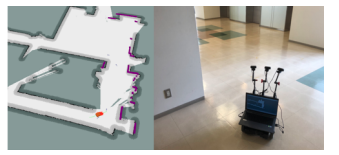
\includegraphics[width = 10cm]{./figs/okada.png}
    \caption{A robot that follows a path using vision based on the proposed method\cite{okada}}
    \label{fig::okada}
\end{figure}


上記の研究により,カメラ画像用いて,ロボットが経路を周回可能であると示されている.


経路を周回 研究の拡張を行う
走行する経路内にFig. \ref{fig::bunki}のような分岐路が含まれる場合,
従来研究では同じ分岐路において
任意のルートへ走行を明確に切り替え.

カメラ画像のみのでは「分岐路をどちらへ進むか」という特定のルート選択を行うために
必要な情報が不足していることが要因と考えられる.
画像のみを入力としたネットワークでは,
分岐路においてネットワークが2つの方向を出力してしまい,左右に車体を向ける振動が発生してしまう事象がDean A. Pomerleauら\cite{pomeru}によって確認されている.

\begin{figure}[h]
    \centering
    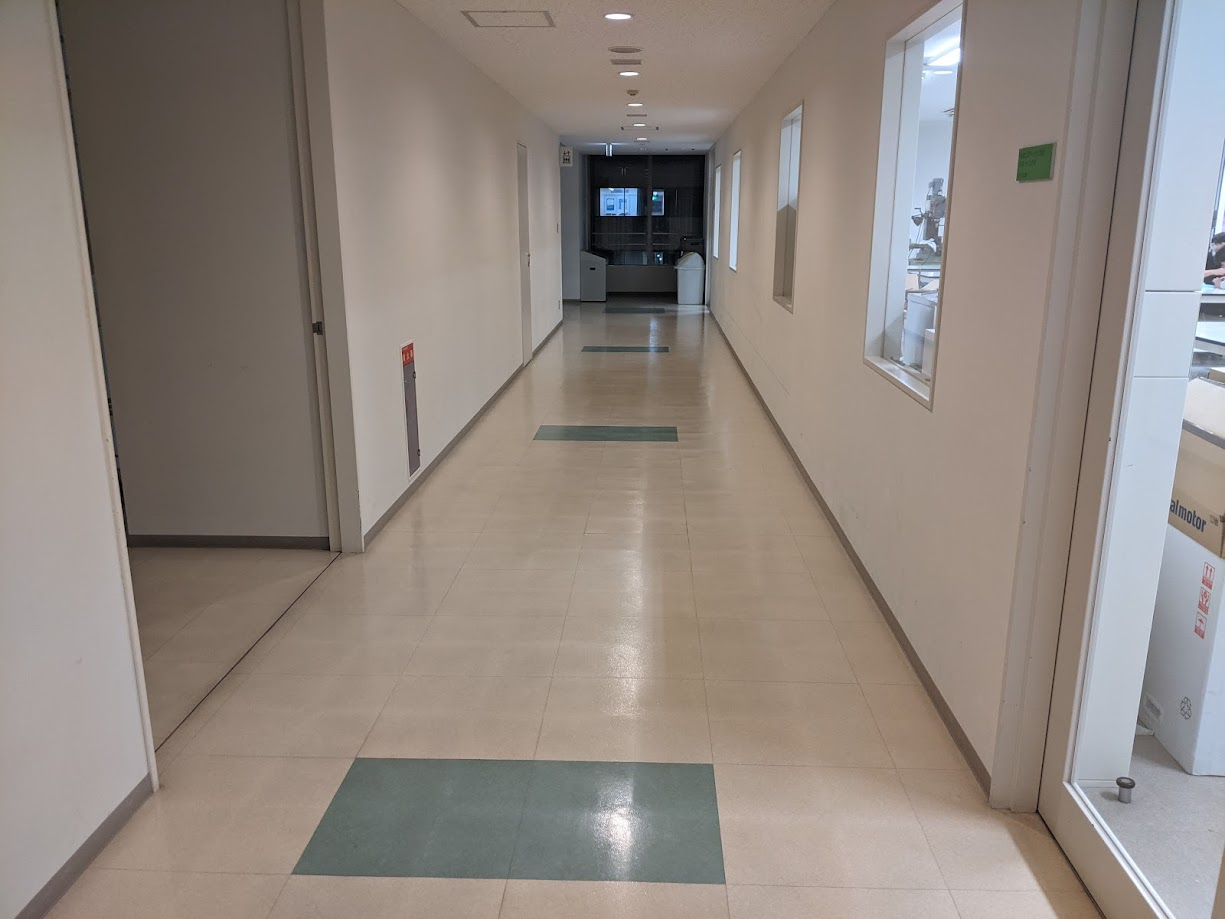
\includegraphics[width = 8cm]{./figs/bunki.jpg}
    \caption{Cross Road}
    \label{fig::bunki}
\end{figure}
\newpage

人間の話分岐路での行動「道案内」
シナリオ
島田シナリオに基づいた
トポロジカルマップとシナリオの
情報を入力へ加えること
\begin{figure}[H]
    \centering
    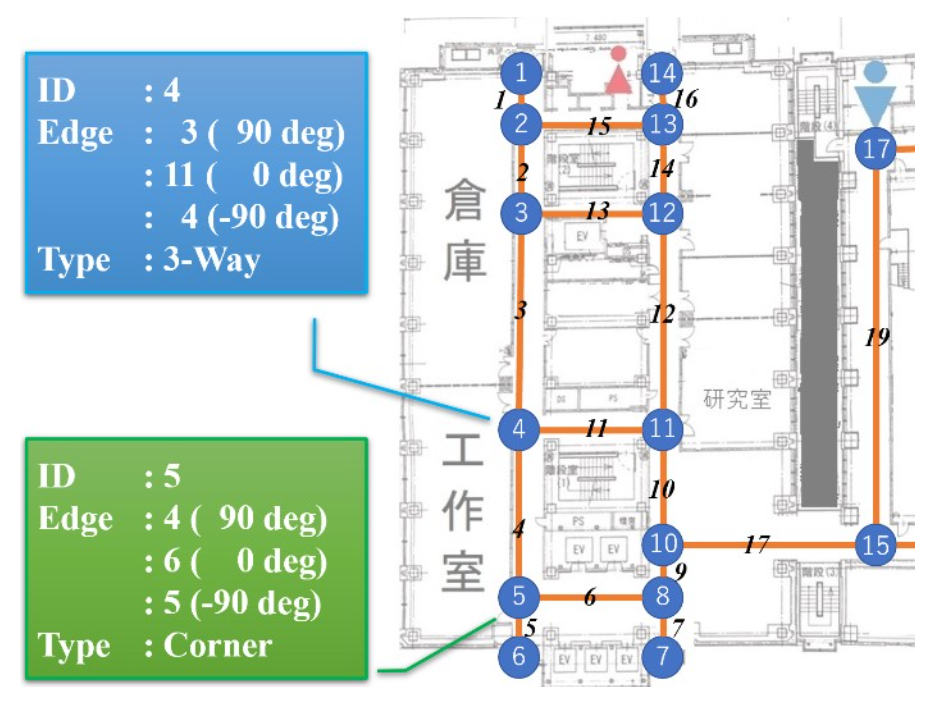
\includegraphics[width = 12cm]{./figs/topo.png}
    \caption{topo\cite{razikon}}
    \label{fig::topo}
\end{figure}
\begin{figure}[H]
    \centering
    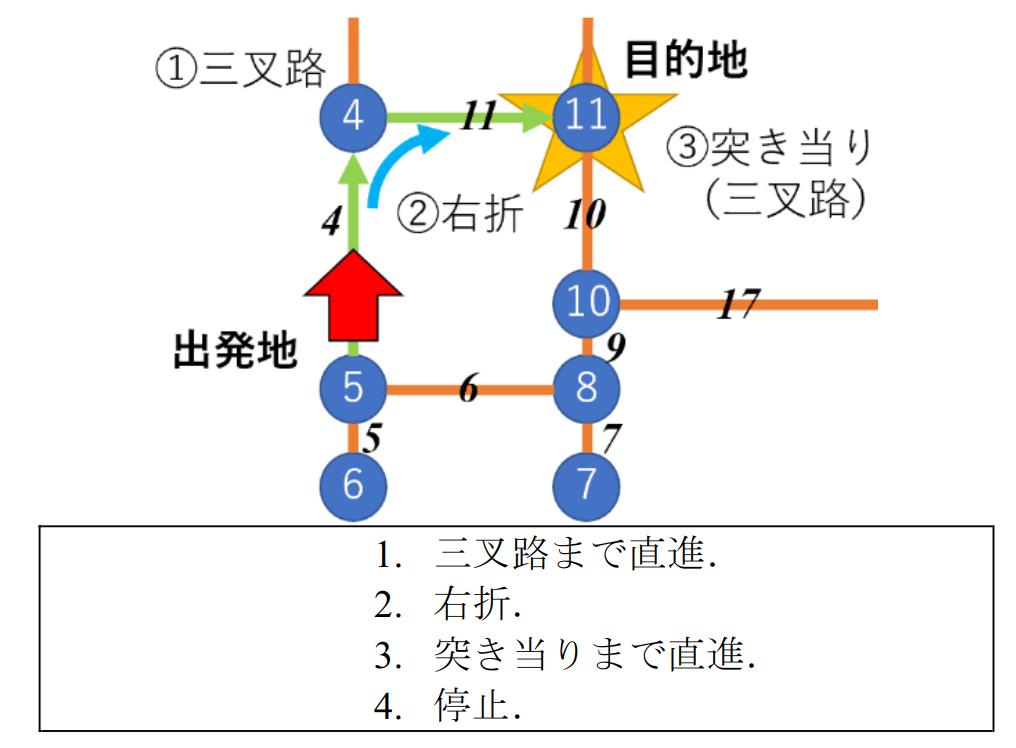
\includegraphics[width = 12cm]{./figs/sina.png}
    \caption{sina\cite{razikon}}
    \label{fig::sina}
\end{figure}
本研究では,\cite{okada}らと島田ら手法を拡張し,
「直進」「左折」「右折」などの目標とする方向情報(本研究では"目標方向"とする)
を追加することで分岐路において特定のルート選択を行う

「カメラ画像と目標方向の情報を用いて,分岐路において任意の走行経路を選択する手法」を提案する.


カメラ画像以外に他の情報を用いて,自律移動を行う研究として
Felipeら\cite{razikon}はカメラ画像と操舵角と加速度の2次元の制御信号と,continue,left,straight,rightの4つのコマンドを入力としたネットワークを
用いてFig. \ref{fig::Conditional_Imitation_Learning}で示すように実環境と都市環境のシミュレータ上で学習器がコマンドに沿った行動が可能であることを
確認している.

\begin{figure}[H]
    \centering
    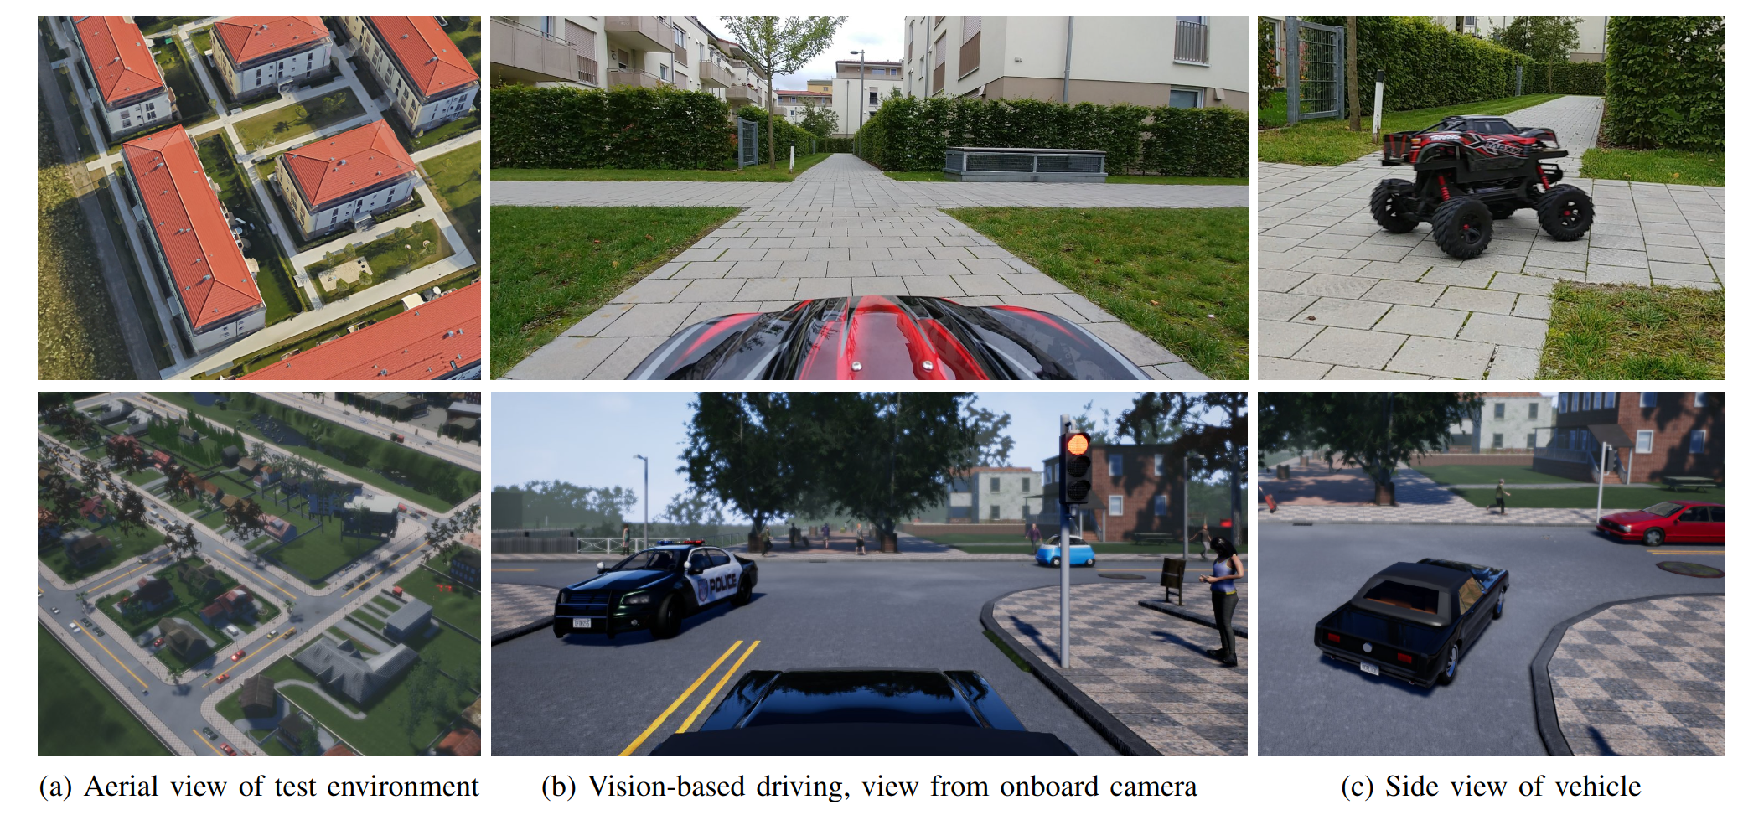
\includegraphics[width = 15cm]{./figs/End-to-end_Driving_via_Conditional_Imitation_Learning.pdf}
    \caption{End-to-end  Driving  via  Conditional  Imitation  Learning from \cite{razikon}}
    \label{fig::Conditional_Imitation_Learning}
\end{figure}

\newpage
また,Seiyaら\cite{nagoya}はFig. \ref{fig::nagoyaabst}で示すように
カメラ画像と目標方向を入力,ステアリング制御信号を出力とするシステムを用いて,右および左に曲がる屋外の軌道を
追跡可能であることを確認している.

\begin{figure}[H]
    \centering
    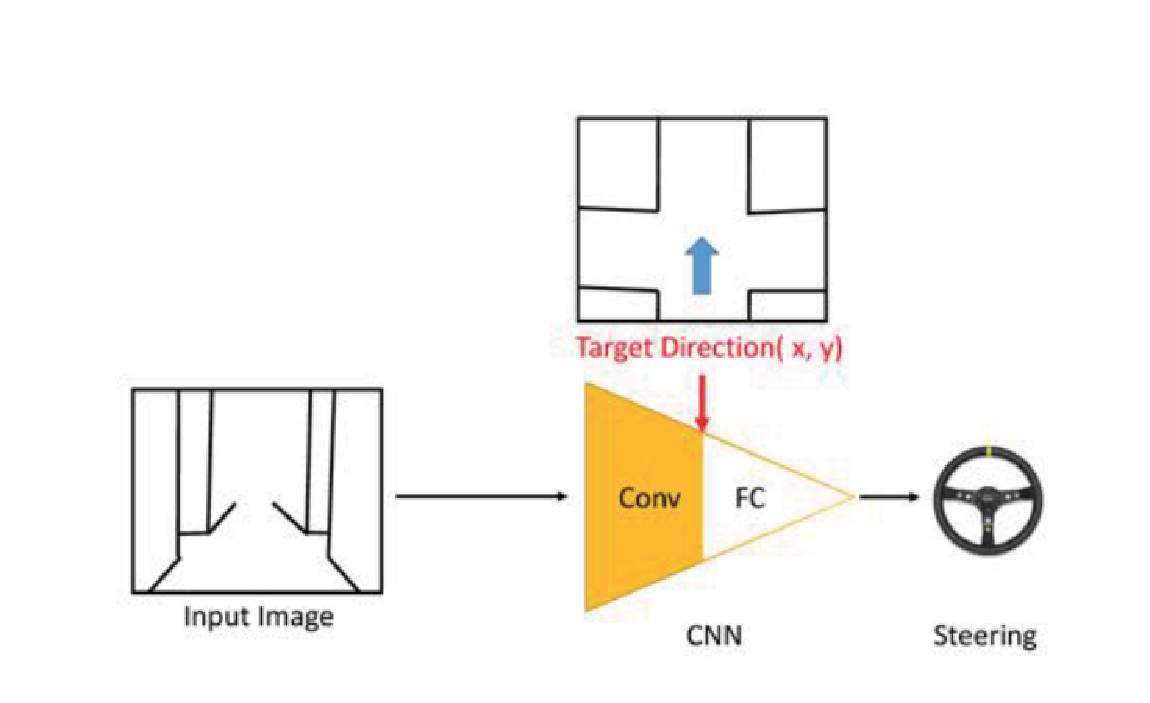
\includegraphics[width = 10cm]{./figs/End-to-End_Navigation_with_Branch_Turning_Support_using_Convolutional_Neural_Network_abst.pdf}
    \caption{Overview of Seiya and others proposed method from \cite{nagoya}}
    \label{fig::nagoyaabst}
\end{figure}


\section{目的}
本研究では,カメラ画像と目標方向を用いたEnd-to-End学習
によるシナリオに基づいたNavigation手法を行う前段階として

カメラ画像と目標方向を入力とする学習器の出力を用いた走行において,分岐路で任意のルートへ走行経路を変更することを目指す.
カメラ画像以外に分岐路での方向指示の情報を追加し,その情報を用いてルート選択が可能であるかの
検証を行う.


\section{論文構成}
1章では,本研究における背景,及び目的を述べた.
2章では,本研究で用いた深層学習の要素技術について述べる.
3章では,本研究で用いた手法と構築したシステムについて述べる.
4章では,構築したシステムを用いた実験を行う.
5章では,本研究の結論を述べる.
